\chapter{KẾT QUẢ THỰC HIỆN}

Chương này trình bày các kết quả đạt được sau quá trình thiết kế, xây dựng và triển khai hệ thống Hardware-in-the-Loop cho kiểm thử phần mềm nhúng. Các kết quả được phân tích theo ba thành phần chính của hệ thống bao gồm: phần mềm HIL, phần mềm giao diện trên máy tính và phần mềm kiểm thử tự động. Qua đó đánh giá mức độ đáp ứng yêu cầu thiết kế cũng như khả năng ứng dụng thực tế của hệ thống.

\section{Kết quả thực hiện phần mềm HIL}

\subsection{Kết quả mô phỏng ngoại vi}
\subsubsection{Kêt quả mô phỏng GPIO}
(thêm bảng số lượng chân GPIO support, các chế độ hoạt động, mức điện áp logic)

\subsubsection{Kết quả mô phỏng ADC}
(thêm bảng số lượng chân ADC support, dải điện áp đo được, độ phân giải ADC)

\subsubsection{Kết quả mô phỏng DAC}
(thêm bảng số lượng chân DAC support, dải điện áp đầu ra, độ phân giải DAC)
(kết quả tạo sóng sine wave, triangle wave)

\subsubsection{Kết quả mô phỏng PWM}
(thêm bảng số lượng chân PWM support, dải tần số, kết quả tạo tín hiệu PWM với tần số và duty cycle khác nhau)

\subsubsection{Kết quả mô phỏng UART}
(thêm bảng số lượng cổng UART support, tốc độ baud rate hỗ trợ, kết quả gửi nhận dữ liệu qua UART)
\subsubsection{Kết quả mô phỏng CAN}
(thêm bảng số lượng cổng CAN support, tốc độ baud rate hỗ trợ, kết quả gửi nhận dữ liệu qua CAN)

\subsection{Kết quả mô phỏng thiết bị}
\subsubsection{Kết quả mô phỏng I2C EEPROM}
(thêm bảng kết quả kiểm thử đọc ghi dữ liệu vào I2C EEPROM mô phỏng, bao gồm địa chỉ, dữ liệu đã ghi, dữ liệu đã đọc và kết quả so sánh)

\subsubsection{Kết quả mô phỏng I2C RTC}
(thêm bảng kết quả kiểm thử thiết lập và đọc thời gian từ RTC mô phỏng, bao gồm thời gian đã thiết lập, thời gian đã đọc và kết quả so sánh)
\subsubsection{Kết quả mô phỏng SPI Flash}
(thêm bảng kết quả kiểm thử đọc ghi dữ liệu vào SPI Flash mô phỏng, bao gồm địa chỉ, dữ liệu đã ghi, dữ liệu đã đọc và kết quả so sánh)

\subsection{Đánh giá kết quả}
(thêm bảng các pin support)

\section{Kết quả thực hiện phần mềm Logic Analyzer trên HIL}

\section{Kết quả thực hiện phần mềm trên máy tính}
Giao diện chính của phần mềm được tổ chức dưới dạng các tab riêng biệt nhằm tăng tính trực quan và thuận tiện trong quá trình sử dụng, bao gồm:
\begin{itemize}
    \item \textbf{Serial Tab}: Cấu hình các  thông số cho Serial port (cổng COM, baudrate).
    \item \textbf{Terminal Tab}: Hỗ trợ giao diện dòng lệnh cho người dùng nhập lệnh thủ công.
    \item \textbf{Memory EMU Tab}: Hỗ trợ người dùng thao tác với thiết bị bộ nhớ mô phỏng trên HIL như SPI Flash và I2C EEPROM.
    \item \textbf{Logic Analyzer Tab}: Hiển thị tín hiệu digital, analog giúp người dùng có thể quan sát và phân tích các tín hiệu như tần số, dạng sóng,...
    \item \textbf{Peripherals Tab}: Hỗ trợ người dùng thao tác với các thiết bị ngoại vi khác như GPIO, ADC, DAC,... để kiểm thử DUT.
\end{itemize}
\begin{figure}[H]
    \centering
    
\includegraphics[width=1\textwidth]{image/PC_GUI.png}
    \caption{Giao diện chính của phần mềm trên máy tính}
    \label{fig:PC_GUI}
\end{figure}

\subsection{Kết quả điều khiển nguồn cho DUT}
Người dùng sẽ được cung cấp các nút nhấn trên giao diện để điều khiển nguồn cho DUT.
\begin{figure}[H]
    \centering
    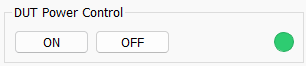
\includegraphics[width=0.7\textwidth]{image/power_on.png}
    \caption{Bật nguồn DUT}
    \label{fig:power_on}
\end{figure}

\begin{figure}[H]
    \centering
    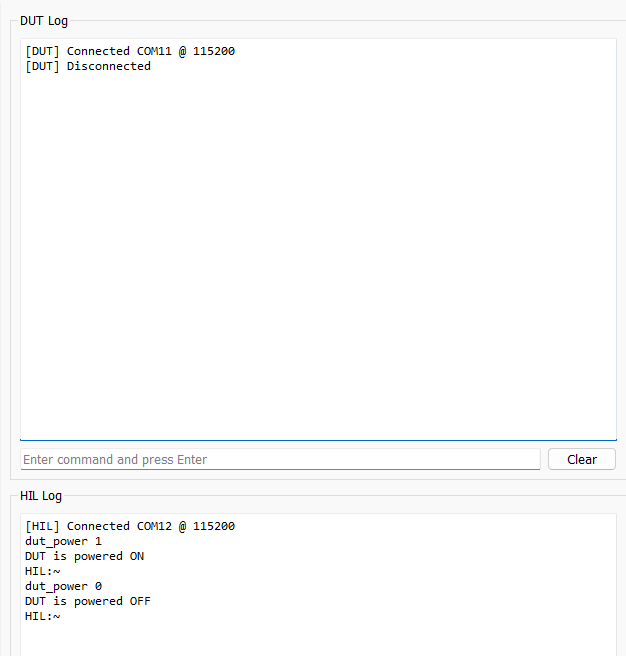
\includegraphics[width=0.7\textwidth]{image/power_off.png}
    \caption{Tắt nguồn DUT}
    \label{fig:power_off}
\end{figure}

\begin{figure}[H]
    \centering
    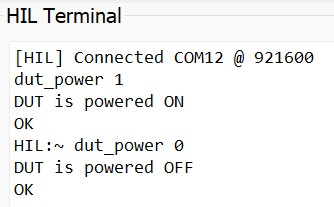
\includegraphics[width=0.5\textwidth]{image/power_app.jpg}
    \caption{Trạng thái nguồn của DUT trong giao diện dòng lệnh}
    \label{fig:power_app}
\end{figure}
\textbf{Nhận xét:} Dựa trên các kết quả từ giao diện UI và giao diện dòng lệnh, có thể thấy nguồn của DUT đã được bật/tắt và trạng thái nguồn được cập nhật qua led trên phần mềm.

\subsection{Kết quả mô phỏng SPI Flash}
Người dùng có thể dùng giao diện dòng lệnh để gửi các command thủ công cho DUT để thực hiện các thao tác đọc ghi dữ liệu vào SPI Flash mô phỏng. Ngoài ra, phần mềm trên máy tính được thiết kế để thực hiện 1 bài kiểm thử tự động để kiểm tra chức năng đọc/ghi dữ liệu của DUT với thiết bị SPI Flash mô phỏng trên hệ thống HIL. Các bước thực hiện bao gồm:
\begin{itemize}
    \item \textbf{Bước 1:} PC gửi lệnh đến \textbf{DUT} đọc ID của thiết bị SPI Flash (HIL đang mô phỏng W25Q128 với ID: 0xEF4018).\\
    \begin{figure}[H]
        \centering
        
\includegraphics[width=0.8\textwidth]{image/spi_read_id.jpg}
        \caption{DUT đọc ID của thiết bị SPI Flash mô phỏng trên HIL}
        \label{fig:spi_read_id}
    \end{figure}

    \item \textbf{Bước 2:} PC gửi lệnh đến \textbf{HIL} để khởi tạo bộ nhớ từ địa chỉ 0 - 255 với giá trị tăng dần từ 0x00 đến 0xFF.\\
    \begin{figure}[H]
        \centering
        
\includegraphics[width=0.8\textwidth]{image/spi_hil_prepare_mem.jpg}
        \caption{HIL khởi tạo bộ nhớ SPI Flash mô phỏng}
        \label{fig:spi_hil_prepare_mem}
    \end{figure}

    \item \textbf{Bước 3:} PC gửi lệnh đến \textbf{DUT}, yêu cầu DUT đọc vào vùng nhớ từ 0 - 255 mà thiết bị SPI Flash mô phỏng trên HIL. Dữ liệu đọc được sẽ được gửi lại PC để so sánh với dữ liệu gốc.\\
    \begin{figure}[H]
        \centering
        
\includegraphics[width=1\textwidth]{image/spi_read_256.jpg}
        \caption{DUT đọc dữ liệu từ SPI Flash mô phỏng}
        \label{fig:spi_read_256}
    \end{figure}

    \item \textbf{Bước 4:} PC gửi lệnh đến \textbf{DUT}, yêu cầu DUT ghi giá trị vào SPI Flash mô phỏng từ địa chỉ 0 - 1023 với giá trị tăng dần từ 0x00 đến 0xFF lặp lại.\\
    \begin{figure}[H]
        \centering
        
\includegraphics[width=0.8\textwidth]{image/spi_write.jpg}
        \caption{DUT ghi dữ liệu vào SPI Flash mô phỏng}
        \label{fig:spi_write}
    \end{figure}

    \item \textbf{Bước 5:} PC gửi lệnh đến \textbf{DUT}, yêu cầu DUT đọc vào vùng nhớ từ 0 - 1023. Dữ liệu đọc được sẽ được gửi lại PC để so sánh với dữ liệu DUT vừa ghi vào.
    \begin{figure}[H]
        \centering
        
\includegraphics[width=1\textwidth]{image/spi_read_after_write.jpg}
        \caption{DUT đọc dữ liệu sau khi ghi vào SPI Flash mô phỏng}
        \label{fig:spi_read_after_write}
    \end{figure}

    \item \textbf{Bước 6:} PC gửi lệnh đến \textbf{DUT} xóa toàn bộ dữ liệu trên SPI Flash mô phỏng.\\
    \begin{figure}[H]
        \centering
        
\includegraphics[width=0.65\textwidth]{image/spi_erase.jpg}
        \caption{DUT xóa dữ liệu trên SPI Flash mô phỏng}
        \label{fig:spi_erase}
    \end{figure}

    \item \textbf{Bước 7:} PC gửi lệnh đến \textbf{DUT}, yêu cầu DUT đọc vào vùng nhớ từ 0 - 1023 (toàn bộ giá trị đều là 0xFF sau khi xóa).
    \begin{figure}[H]
        \centering
        
\includegraphics[width=1\textwidth]{image/spi_read_after_erase.jpg}
        \caption{DUT đọc dữ liệu sau khi xóa trên SPI Flash mô phỏng}
        \label{fig:spi_read_after_erase}
    \end{figure}
\end{itemize}

Sau khi hoàn thành các bước kiểm thử, kết quả sẽ được hiển thị trên giao diện chính của phần mềm PC như Hình \ref{fig:spi_test_result}.\\

\begin{figure}[H]
    \centering
    
\includegraphics[width=0.7\textwidth]{image/spi_result.jpg}
    \caption{Kết quả kiểm thử SPI Flash trên phần mềm PC}
    \label{fig:spi_test_result}
\end{figure}
Kết quả kiểm thử cho thấy DUT đã thực hiện chính xác các thao tác đọc, ghi và xóa dữ liệu trên thiết bị SPI Flash mô phỏng bởi hệ thống HIL. 
Dữ liệu đọc được từ DUT hoàn toàn khớp với dữ liệu gốc đã được khởi tạo trên HIL, chứng tỏ tính đúng đắn của quá trình giao tiếp và xử lý dữ liệu giữa DUT và HIL.


\section{Kết quả thực hiện phần mềm kiểm thử tự động trên máy tính}

\subsection{Tổ chức thư mục}
Để thuận tiện cho việc phát triển, mở rộng và bảo trì hệ thống kiểm thử tự động, cấu trúc thư mục của dự án được tổ chức theo hướng phân tách rõ ràng giữa các thành phần kiểm thử, thư viện keyword, tài nguyên dùng chung và kết quả thực thi. 

Hệ thống kiểm thử được xây dựng dựa trên Robot Framework kết hợp với các thư viện Python nhằm hỗ trợ giao tiếp với HIL và Logic Analyzer. Cấu trúc thư mục tổng quát của hệ thống được trình bày như Hình \ref{fig:robot_folder_structure}.

\begin{figure}[H]
    \centering
    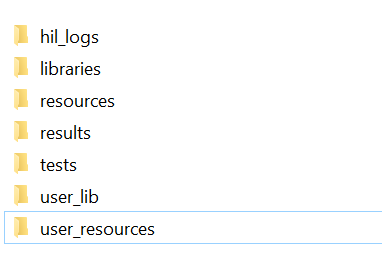
\includegraphics[width=0.8\textwidth]{image/robot_folder_structure.png}
    \caption{Lưu đồ giải thuật kiểm tra kết nối HIL và DUT}
    \label{fig:robot_folder_structure}
\end{figure}

Trong đó, các thư mục chính của hệ thống HIL bao gồm:

\begin{itemize}
    \item \textbf{hil\_logs/}: Ghi lại các log chi tiết của quá trình giao tiếp giữa Robot Framework với hệ thống HIL, bao gồm các lệnh đã gửi, phản hồi nhận được và trạng thái hoạt động của HIL trong suốt quá trình kiểm thử mỗi lần chạy.
    \item \textbf{libraries/}: Chứa các tập tin định nghĩa keyword dùng chung trong Robot Framework. Các keyword này được sử dụng để xây dựng các bước kiểm thử ở mức cao, giúp test case trở nên trực quan và thân thiện với người dùng hơn. Các thư viện này cũng đóng vai trò là lớp giao tiếp trung gian giữa Robot Framework với hệ thống HIL và Logic Analyzer, giúp ẩn đi các chi tiết mức thấp và cung cấp các thao tác đơn giản để điều khiển hệ thống.
    \item \textbf{resources/}: Chứa các tài nguyên dùng chung như biến cấu hình, thông số giao tiếp,... cho HIL, được sử dụng trong nhiều bài kiểm thử khác nhau.
    \item \textbf{results/}: Chứa kết quả sau khi thực hiện kiểm thử bao gồm file báo cáo tổng hợp, file log chi tiết và các dữ liệu phục vụ cho việc đánh giá kết quả kiểm thử.
    \item \textbf{tests/}: Chứa các tập tin kiểm thử được xây dựng bằng Robot Framework. Hệ thống hiện đã cung cấp sẵn các bài kiểm thử mẫu cho các ngoại vi và thiết bị mô phỏng được hỗ trợ trên HIL nhằm giúp người dùng tham khảo và phát triển thêm các kịch bản kiểm thử mới.

\end{itemize}

Các thư mục do người dùng tạo ra bao gồm:

\begin{itemize}
    \item \textbf{user\_lib/}: Chứa các tập tin định nghĩa keyword do người dùng tự định nghĩa để giao tiếp với hệ thống DUT.
    \item \textbf{user\_resources/}: Chứa các tài nguyên dùng chung như biến cấu hình, thông số giao tiếp,... cho DUT, được sử dụng trong nhiều bài kiểm thử khác nhau.

\end{itemize}

Với cách tổ chức này, các thành phần trong hệ thống được phân tách rõ ràng giữa phần kiểm thử, phần xử lý giao tiếp phần cứng và phần kết quả đầu ra. Điều này giúp việc phát triển thêm các bài kiểm thử mới, mở rộng hỗ trợ cho các ngoại vi khác cũng như tái sử dụng framework cho nhiều DUT khác nhau trở nên thuận tiện hơn.

\subsection{Các keyword hỗ trợ trong hệ thống kiểm thử}

Các keyword được xây dựng trong hệ thống kiểm thử tự động đóng vai trò là lớp giao tiếp trung gian giữa Robot Framework với hệ thống HIL và Logic Analyzer. Thay vì thao tác trực tiếp với các lệnh điều khiển mức thấp, người phát triển chỉ cần sử dụng các keyword tương ứng để xây dựng các test case theo dạng mô tả hành vi kiểm thử.

Bảng \ref{tab:hil_keywords} và Bảng \ref{tab:la_keywords} trình bày các keyword tiêu biểu được hỗ trợ trong hệ thống kiểm thử.

\renewcommand{\arraystretch}{1.3}

\begin{longtable}{|p{4.8cm}|p{8.7cm}|}
\caption{Các keyword hỗ trợ bởi thư viện HIL}
\label{tab:hil_keywords} \\

\hline
\textbf{Keyword} & \textbf{Chức năng} \\
\hline
\endfirsthead

\hline
\textbf{Keyword} & \textbf{Chức năng} \\
\hline
\endhead

\multicolumn{2}{|c|}{\textbf{Kết nối và điều khiển DUT}} \\
\hline

Connect HIL
& Thiết lập kết nối giữa PC và hệ thống HIL thông qua USB serial. \\
\hline

Disconnect HIL
& Ngắt kết nối giữa PC và hệ thống HIL. \\
\hline

Verify HIL Alive
& Kiểm tra khả năng phản hồi và trạng thái hoạt động của HIL. \\
\hline

HIL Power DUT On
& Cấp nguồn cho DUT thông qua HIL. \\
\hline

HIL Power DUT Off
& Ngắt nguồn DUT thông qua HIL. \\
\hline

HIL Power DUT Cycle
& Thực hiện reset nguồn DUT bằng cách tắt và cấp nguồn lại. \\
\hline

HIL Flash Firmware for DUT
& Nạp firmware cho DUT thông qua chế độ DFU sử dụng STM32CubeProgrammer CLI. \\
\hline

\multicolumn{2}{|c|}{\textbf{GPIO}} \\
\hline

HIL Set GPIO
& Thiết lập trạng thái logic cho chân GPIO mô phỏng. \\
\hline

HIL Read GPIO
& Đọc trạng thái logic của chân GPIO từ DUT. \\
\hline

\multicolumn{2}{|c|}{\textbf{UART}} \\
\hline

HIL Init UART
& Khởi tạo giao tiếp UART trên HIL. \\
\hline

HIL Send UART String
& Gửi chuỗi dữ liệu UART đến DUT. \\
\hline

HIL Read UART Data
& Đọc dữ liệu UART phản hồi từ DUT. \\
\hline

HIL Verify UART String
& Kiểm tra tính đúng đắn của chuỗi UART nhận được. \\
\hline

\multicolumn{2}{|c|}{\textbf{CAN}} \\
\hline

HIL Send CAN Buffer
& Gửi dữ liệu CAN dạng buffer đến DUT. \\
\hline

HIL Send CAN String
& Gửi chuỗi dữ liệu thông qua giao tiếp CAN. \\
\hline

HIL Read CAN Data
& Đọc dữ liệu phản hồi từ giao tiếp CAN. \\
\hline

HIL Verify CAN String Data
& Kiểm tra tính đúng đắn của chuỗi dữ liệu CAN nhận được. \\
\hline

\multicolumn{2}{|c|}{\textbf{I2C EEPROM}} \\
\hline

HIL Init EEPROM
& Khởi tạo EEPROM mô phỏng trên bus I2C. \\
\hline

HIL Deinit EEPROM
& Giải phóng EEPROM mô phỏng khỏi hệ thống HIL. \\
\hline

HIL Find EEPROM
& Kiểm tra sự tồn tại của EEPROM trên bus I2C. \\
\hline

HIL Activate I2C Device
& Kích hoạt thiết bị I2C mô phỏng trên HIL. \\
\hline

\multicolumn{2}{|c|}{\textbf{I2C RTC}} \\
\hline

HIL Init RTC
& Khởi tạo RTC mô phỏng trên bus I2C. \\
\hline

HIL Prepare RTC Time
& Thiết lập thời gian cho RTC mô phỏng. \\
\hline

HIL Get RTC Time
& Đọc giá trị thời gian hiện tại từ RTC mô phỏng. \\
\hline

HIL Set RTC Date
& Thiết lập ngày tháng cho RTC mô phỏng. \\
\hline

HIL Get RTC Date
& Đọc ngày tháng hiện tại từ RTC mô phỏng. \\
\hline

\multicolumn{2}{|c|}{\textbf{SPI Flash}} \\
\hline

HIL Prepare SPI Flash Data
& Chuẩn bị dữ liệu mẫu trong SPI Flash để DUT thực hiện đọc dữ liệu. \\
\hline

\multicolumn{2}{|c|}{\textbf{ADC/DAC}} \\
\hline

HIL Read ADC Voltage
& Đọc giá trị điện áp ADC đo được từ HIL. \\
\hline

HIL Set DAC Voltage
& Thiết lập điện áp DAC đầu ra của HIL. \\
\hline

HIL Generate Sine Wave
& Tạo tín hiệu sine wave phục vụ kiểm thử DAC hoặc ADC. \\
\hline

HIL Stop Sine Wave
& Dừng phát tín hiệu sine wave. \\
\hline

HIL Generate Triangle Wave
& Tạo tín hiệu triangle wave phục vụ kiểm thử DAC hoặc ADC. \\
\hline

HIL Stop Triangle Wave
& Dừng phát tín hiệu triangle wave. \\
\hline

\end{longtable}

\begin{table}[H]
\centering
\caption{Các keyword hỗ trợ bởi thư viện Logic Analyzer}
\label{tab:la_keywords}
\renewcommand{\arraystretch}{1.3}

\begin{tabular}{|p{5cm}|p{8.5cm}|}
\hline
\textbf{Keyword} & \textbf{Chức năng} \\
\hline

Connect Logic Analyzer
& Thiết lập kết nối với Logic Analyzer thông qua USB serial. \\
\hline

Disconnect Logic Analyzer
& Ngắt kết nối với Logic Analyzer. \\
\hline

LA Read Data
& Thu thập dữ liệu tín hiệu từ Logic Analyzer. \\
\hline

LA Verify Sine Wave
& Phân tích FFT để xác minh tín hiệu analog dạng sine wave và kiểm tra tần số tín hiệu. \\
\hline

LA Verify Pulse Wave
& Phân tích tín hiệu số nhằm xác định tần số và duty cycle của tín hiệu PWM hoặc pulse wave. \\
\hline

LA Verify Triangle Wave
& Phân tích phổ hài để xác minh tín hiệu analog dạng triangle wave. \\
\hline

\end{tabular}
\end{table}

\subsection{Ví dụ test case kiểm thử}

Trong Robot Framework, một tập tin kiểm thử được tổ chức thành nhiều thành phần nhằm mô tả tài nguyên sử dụng, biến cấu hình và các bước kiểm thử. Việc tổ chức theo cấu trúc này giúp các bài kiểm thử trở nên trực quan, dễ mở rộng và thuận tiện cho việc tái sử dụng trong nhiều dự án khác nhau.

Để minh họa cho cách xây dựng một bài kiểm thử trong hệ thống, luận văn sử dụng ví dụ kiểm thử chức năng đọc điện áp ADC của DUT thông qua tín hiệu DAC được tạo bởi HIL. Nội dung file kiểm thử được trình bày như Hình \ref{fig:robot_adc_testcase}.

\begin{figure}[H]
    \centering
    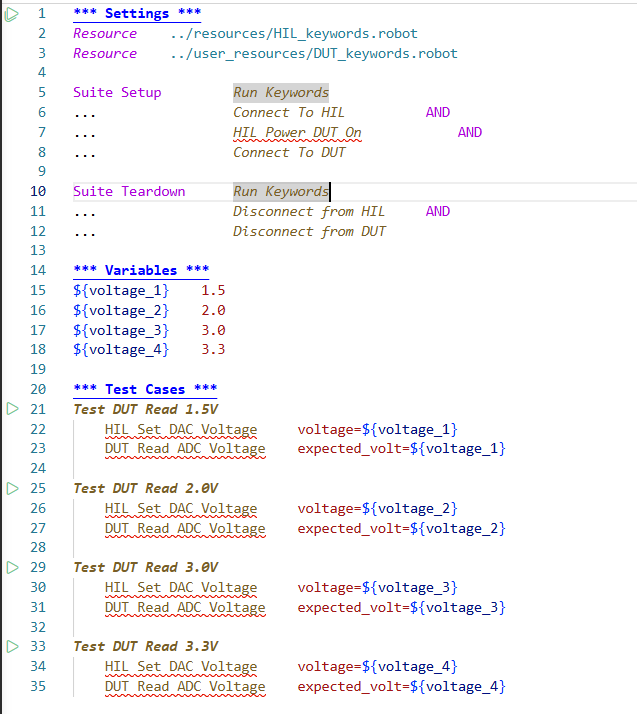
\includegraphics[width=0.8\textwidth]{image/robot_adc_testcase.png}
    \caption{í dụ file kiểm thử ADC bằng Robot Framework}
    \label{fig:robot_adc_testcase}
\end{figure}

Trong Robot Framework, phần \textbf{Settings} được sử dụng để khai báo các tài nguyên, thư viện và cấu hình chung cho toàn bộ file kiểm thử. 

Trong ví dụ trên, hai dòng lệnh:

\begin{lstlisting}[language={}]
Resource    ../resources/HIL_keywords.robot
Resource    ../user_resources/DUT_keywords.robot
\end{lstlisting}

được sử dụng để import các tập tin resource chứa các keyword phục vụ cho quá trình kiểm thử.

Trong đó:

\begin{itemize}

    \item \textbf{HIL\_keywords.robot}: Chứa các keyword phục vụ điều khiển hệ thống HIL như điều khiển DAC, GPIO, UART, CAN hoặc các thiết bị mô phỏng ngoại vi.

    \item \textbf{DUT\_keywords.robot}: Chứa các keyword do người dùng xây dựng để giao tiếp và kiểm tra DUT, ví dụ như đọc dữ liệu UART từ DUT hoặc xác minh giá trị ADC mà DUT đo được.

\end{itemize}

Việc tách các keyword thành các file resource riêng giúp tăng khả năng tái sử dụng và giảm sự phụ thuộc trực tiếp giữa các test case với phần xử lý giao tiếp mức thấp.

Ngoài ra, phần \textbf{Settings} còn định nghĩa các bước khởi tạo và giải phóng tài nguyên thông qua \textit{Suite Setup} và \textit{Suite Teardown}.

\begin{itemize}

    \item \textbf{Suite Setup}: Là tập hợp các thao tác được thực hiện một lần trước khi bắt đầu chạy toàn bộ các test case trong file kiểm thử.

\end{itemize}

Trong ví dụ trên, \textit{Suite Setup} thực hiện các bước:

\begin{enumerate}

    \item Thiết lập kết nối giữa máy tính và hệ thống HIL.
    
    \item Cấp nguồn cho DUT thông qua HIL.
    
    \item Thiết lập kết nối giao tiếp với DUT.

\end{enumerate}

Nhờ đó, toàn bộ môi trường kiểm thử được chuẩn bị tự động trước khi thực hiện các bài kiểm thử.

\begin{itemize}

    \item \textbf{Suite Teardown}: Là tập hợp các thao tác được thực hiện sau khi hoàn thành toàn bộ quá trình kiểm thử nhằm giải phóng tài nguyên và đưa hệ thống về trạng thái an toàn.

\end{itemize}

Trong ví dụ trên, \textit{Suite Teardown} thực hiện đóng kết nối với HIL và DUT sau khi tất cả các test case đã chạy xong.

Phần \textbf{Variables} được sử dụng để khai báo các biến dùng chung trong file kiểm thử. Các giá trị điện áp như 1.5V, 2.0V, 3.0V và 3.3V được lưu dưới dạng biến nhằm giúp việc thay đổi tham số kiểm thử trở nên thuận tiện hơn và tăng khả năng tái sử dụng test case.

Phần \textbf{Test Cases} chứa các kịch bản kiểm thử cụ thể. Mỗi test case trong ví dụ trên thực hiện quy trình kiểm thử ADC của DUT theo các bước:

\begin{enumerate}

    \item HIL phát ra mức điện áp tương ứng thông qua DAC.
    
    \item DUT thực hiện đọc giá trị điện áp bằng ADC.
    
    \item DUT gửi kết quả đo được về máy tính.
    
    \item Keyword kiểm thử thực hiện so sánh giá trị nhận được với giá trị mong đợi để xác định kết quả đạt hoặc không đạt.

\end{enumerate}

\subsection{Quy trình thực hiện kiểm thử tự động}
\subsubsection{Thực hiện một bài kiểm thử}

Đối với một bài kiểm thử đơn lẻ, người dùng có thể thực hiện chạy trực tiếp file test case bằng lệnh Robot Framework tương ứng.

Ví dụ:

\begin{lstlisting}[language=bash]
robot -d results .\tests\05__analog_test.robot
\end{lstlisting}

Sau khi thực thi lệnh, Robot Framework sẽ tự động:

\begin{itemize}

    \item Phân tích file kiểm thử.
    
    \item Import các resource và keyword cần thiết.
    
    \item Thực hiện các bước trong \textit{Suite Setup}.
    
    \item Chạy lần lượt các test case trong file.
    
    \item Đánh giá kết quả đạt hoặc không đạt.
    
    \item Thực hiện \textit{Suite Teardown}.
    
    \item Sinh báo cáo kiểm thử sau khi hoàn thành.

\end{itemize}

Trong quá trình thực hiện, trạng thái của từng test case sẽ được hiển thị trực tiếp trên terminal nhằm hỗ trợ người dùng theo dõi tiến trình kiểm thử.

\begin{figure}[H]
    \centering
    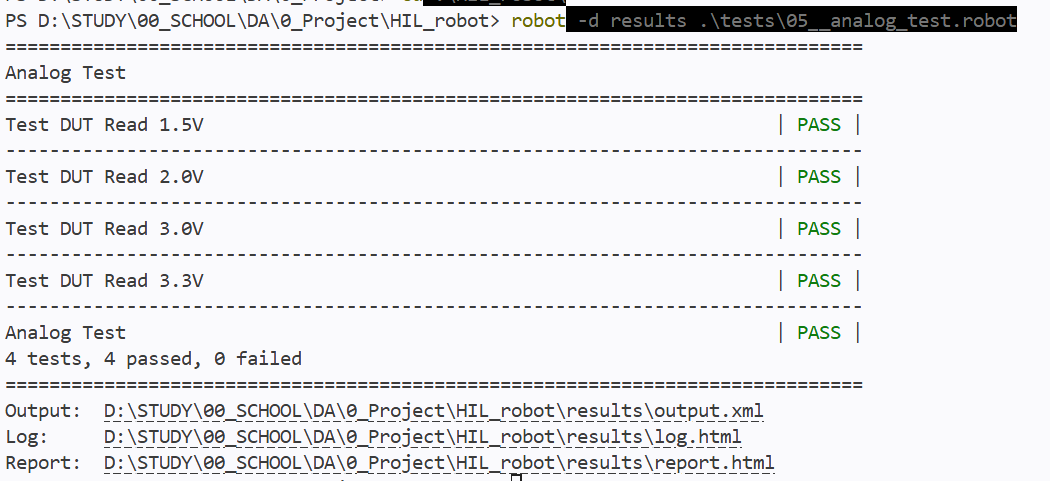
\includegraphics[width=0.85\textwidth]{image/robot_terminal.png}
    \caption{Trạng thái thực hiện kiểm thử được hiển thị trên terminal}
    \label{fig:robot_terminal}
\end{figure}

\subsubsection{Thực hiện nhiều bài kiểm thử liên tiếp}

Ngoài việc thực hiện một bài kiểm thử đơn lẻ, hệ thống còn hỗ trợ chạy nhiều file kiểm thử liên tiếp nhằm phục vụ cho kiểm thử hồi quy firmware.

Người dùng có thể thực hiện kiểm thử toàn bộ thư mục chứa các test case bằng lệnh:

\begin{lstlisting}[language=bash]
robot -d results .\tests\
\end{lstlisting}

Khi đó, Robot Framework sẽ tự động tìm kiếm tất cả các file kiểm thử trong thư mục \textit{tests/} và thực hiện tuần tự từng bài kiểm thử.

Cơ chế này cho phép:

\begin{itemize}

    \item Kiểm thử đồng thời nhiều chức năng của DUT.
    
    \item Tự động hóa quá trình kiểm thử firmware sau mỗi lần cập nhật.
    
    \item Giảm thời gian thao tác thủ công của người phát triển.
    
    \item Hỗ trợ kiểm thử hồi quy nhằm phát hiện lỗi phát sinh sau khi thay đổi firmware.

\end{itemize}

Sau khi hoàn thành, Robot Framework sẽ tự động tổng hợp kết quả của toàn bộ các bài kiểm thử và sinh báo cáo thống kê tổng quát.

\subsubsection{Thiết lập thứ tự thực hiện các bài kiểm thử}

Trong một số trường hợp, các bài kiểm thử cần được thực hiện theo một trình tự xác định nhằm đảm bảo trạng thái hoạt động phù hợp của DUT hoặc phục vụ cho quá trình kiểm thử hồi quy.

Để hỗ trợ điều này, hệ thống cho phép người dùng tổ chức thứ tự thực hiện test case theo nhiều phương pháp khác nhau.

Một phương pháp đơn giản là sử dụng tiền tố số thứ tự (\textit{numeric prefix}) trong tên file kiểm thử. Ví dụ:

\begin{lstlisting}[language={}]
tests/
|-- 01_gpio.robot
|-- 02_adc.robot
|-- 03_uart.robot
|-- 04_can.robot
\end{lstlisting}

Khi thực hiện chạy toàn bộ thư mục kiểm thử, Robot Framework sẽ thực hiện các file theo thứ tự tên file, từ đó đảm bảo đúng trình tự kiểm thử mong muốn.

Ngoài ra, hệ thống cũng hỗ trợ xây dựng một file điều phối kiểm thử dùng để quy định rõ trình tự thực hiện các bài kiểm thử. File này đóng vai trò như một tập kiểm thử tổng hợp (\textit{test suite}) dùng để gọi lần lượt các test case hoặc các nhóm kiểm thử khác nhau.

Phương pháp này phù hợp với các hệ thống có số lượng bài kiểm thử lớn hoặc cần xây dựng các kịch bản kiểm thử chuyên biệt cho từng phiên bản firmware.

Nhờ khả năng tổ chức linh hoạt này, người dùng có thể dễ dàng quản lý quá trình kiểm thử tự động, đồng thời đảm bảo các bài kiểm thử được thực hiện theo đúng trình tự yêu cầu của hệ thống.

\subsection{Kết quả sinh báo cáo}

Sau khi hoàn thành quá trình kiểm thử tự động, Robot Framework sẽ tự động sinh ra các tập tin báo cáo phục vụ cho việc theo dõi, phân tích và đánh giá kết quả kiểm thử.

Các tập tin kết quả được lưu trong thư mục \textit{results/} của hệ thống kiểm thử. Trong đó, các tập tin quan trọng bao gồm:

\begin{itemize}

    \item \textbf{report.html}: Báo cáo tổng hợp kết quả kiểm thử.
    
    \item \textbf{log.html}: File log chi tiết quá trình thực hiện từng keyword và test case.
    
    \item \textbf{output.xml}: File dữ liệu kết quả ở định dạng XML phục vụ cho việc lưu trữ hoặc tích hợp với các hệ thống CI/CD trong tương lai.
\end{itemize}

Hình \ref{fig:robot_report_success} trình bày giao diện báo cáo khi toàn bộ bài kiểm thử thực hiện thành công.

\begin{figure}[H]
    \centering
    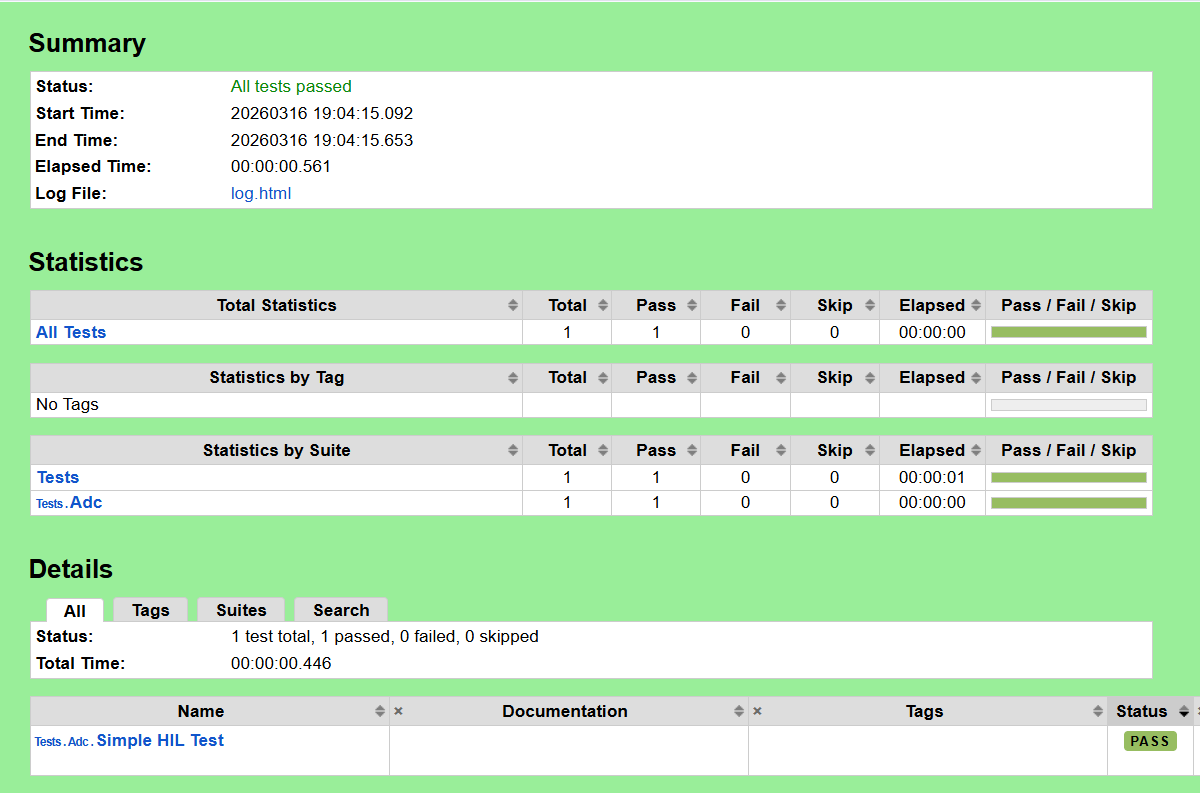
\includegraphics[width=0.85\textwidth]{image/robot_report_success.png}
    \caption{Báo cáo kiểm thử khi toàn bộ test case đạt}
    \label{fig:robot_report_success}
\end{figure}

Trong trường hợp tất cả các điều kiện kiểm thử đều thỏa mãn, Robot Framework sẽ đánh dấu trạng thái \textit{PASS} cho từng test case cũng như toàn bộ test suite. Báo cáo đồng thời cung cấp thông tin về:

\begin{itemize}
    \item Số lượng test case đạt và không đạt.
    \item Thời gian thực hiện kiểm thử.
    \item Tỷ lệ thành công của toàn bộ bài kiểm thử.
    \item Tên các test case đã thực hiện.
\end{itemize}

Ngược lại, khi xuất hiện lỗi trong quá trình kiểm thử hoặc kết quả đo được không đúng với giá trị mong đợi, Robot Framework sẽ đánh dấu trạng thái \textit{FAIL}. Ví dụ báo cáo khi bài kiểm thử thất bại được trình bày như Hình \ref{fig:robot_report_fail}.

\begin{figure}[H]
    \centering
    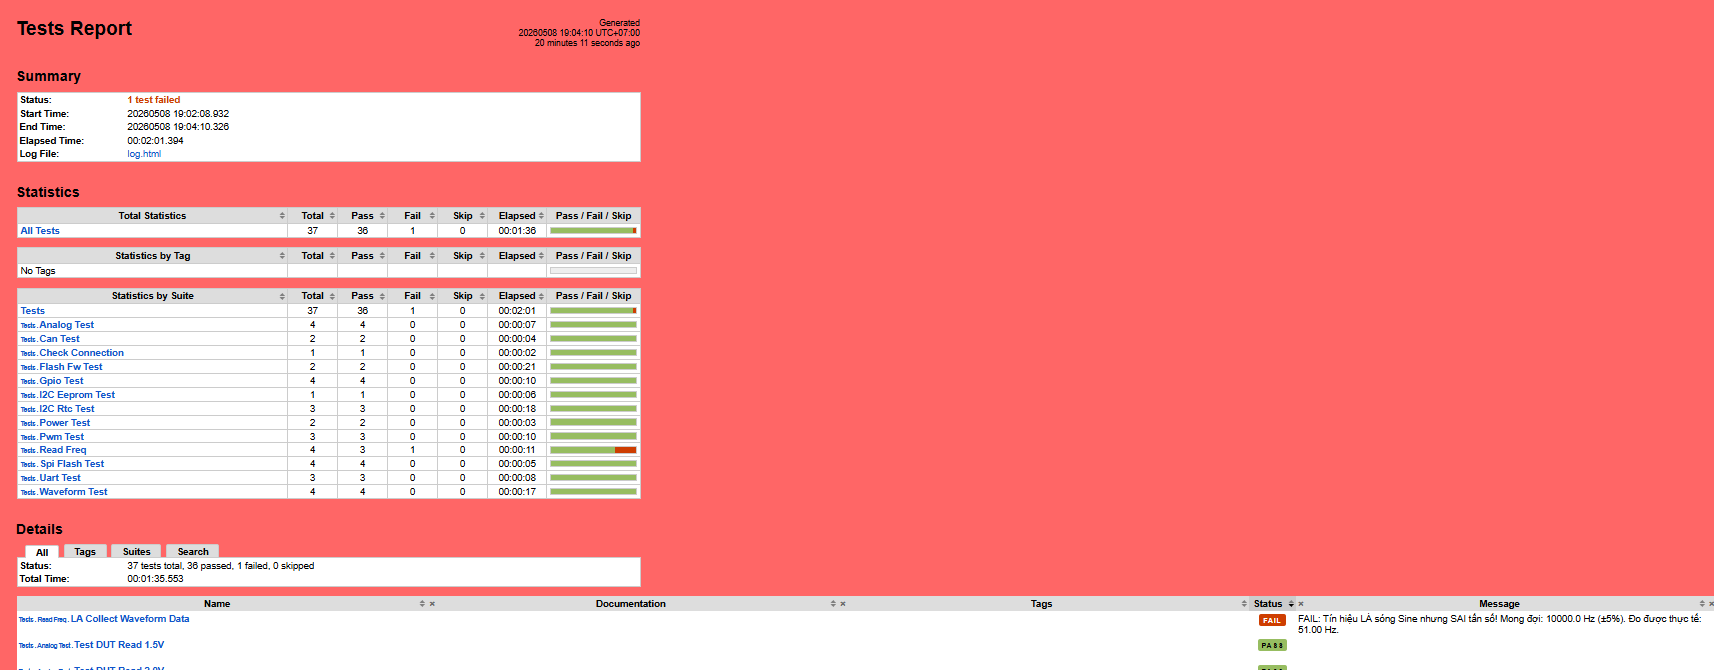
\includegraphics[width=0.85\textwidth]{image/robot_report_fail.png}
    \caption{Báo cáo kiểm thử khi toàn bộ test case không đạt}
    \label{fig:robot_report_fail}
\end{figure}

Thông qua báo cáo này, người phát triển có thể nhanh chóng xác định test case xảy ra lỗi và tiến hành phân tích nguyên nhân.

Ngoài báo cáo tổng hợp, hệ thống còn sinh file \textit{log.html} nhằm ghi lại chi tiết toàn bộ quá trình thực hiện kiểm thử. Nội dung file log được trình bày như Hình \ref{fig:robot_log_file}.

\begin{figure}[H]
    \centering
    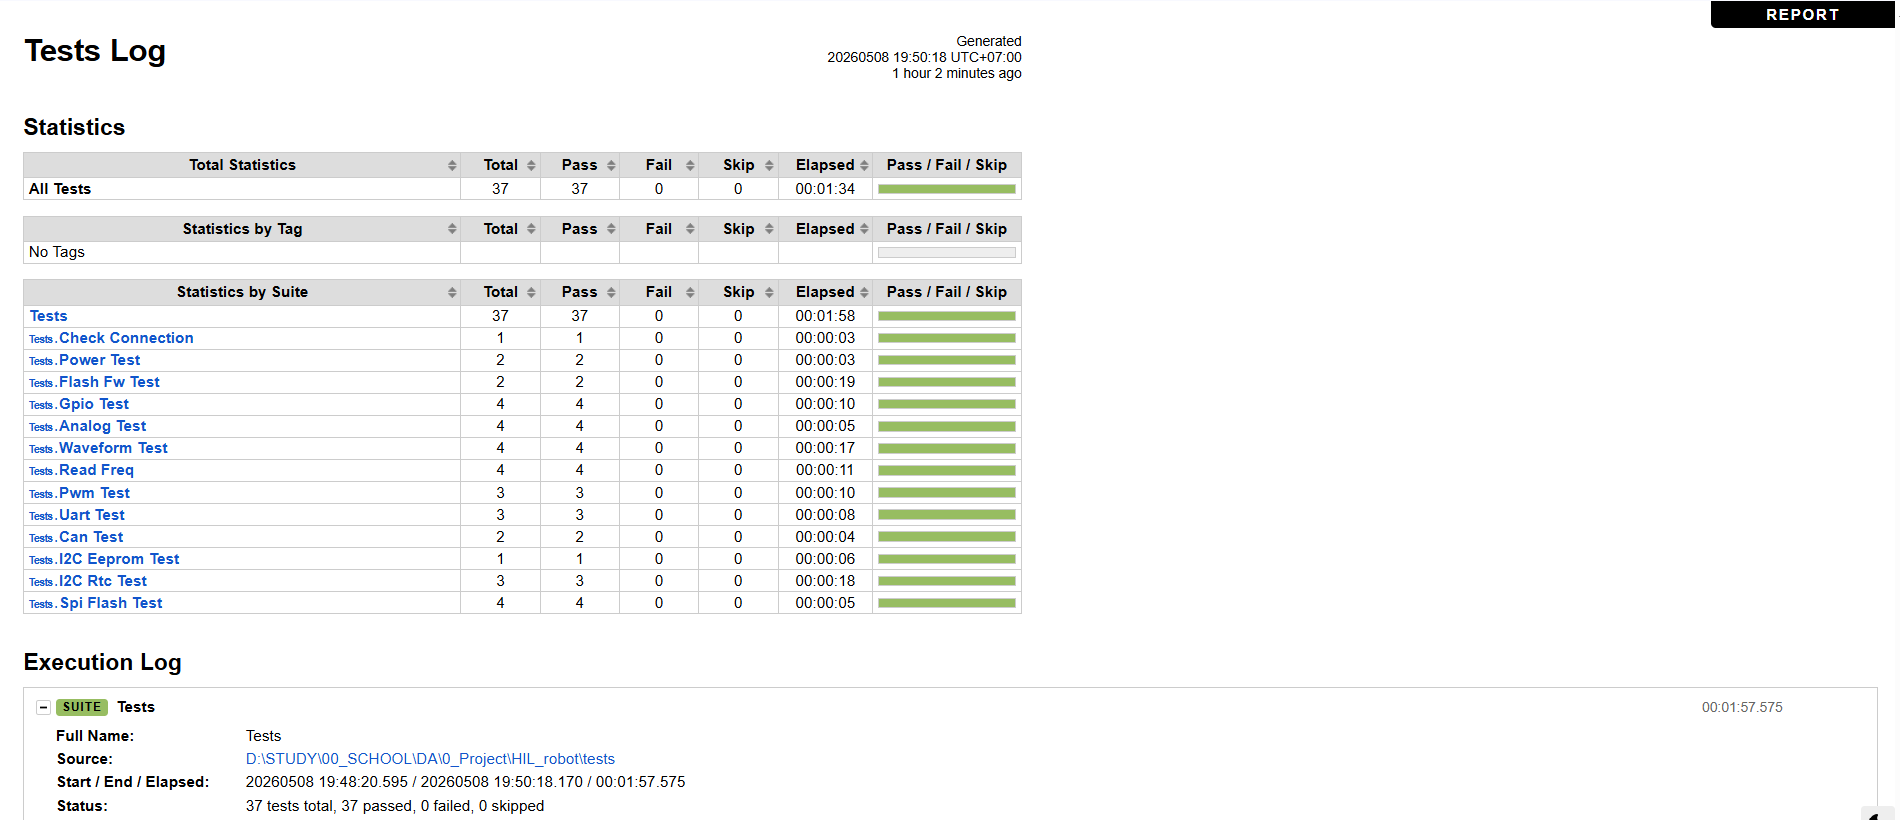
\includegraphics[width=0.85\textwidth]{image/robot_log.png}
    \caption{File log chi tiết của Robot Framework}
    \label{fig:robot_log_file}
\end{figure}

File log cung cấp thông tin chi tiết cho từng bước thực hiện bao gồm:

\begin{itemize}
    \item Các keyword đã được gọi.
    \item Tham số đầu vào của keyword.
    \item Dữ liệu phản hồi từ DUT hoặc HIL.
    \item Thời gian thực hiện từng bước.
    \item Thông báo lỗi và nguyên nhân gây lỗi nếu có.
\end{itemize}

Nhờ đó, người phát triển có thể dễ dàng theo dõi luồng thực thi của hệ thống và hỗ trợ quá trình phân tích lỗi firmware.

Bên cạnh đó, Robot Framework cũng sinh file \textit{output.xml} chứa toàn bộ kết quả kiểm thử ở dạng dữ liệu có cấu trúc. Ví dụ file \textit{output.xml} được trình bày như Hình \ref{fig:robot_output_xml}.

\begin{figure}[H]
    \centering
    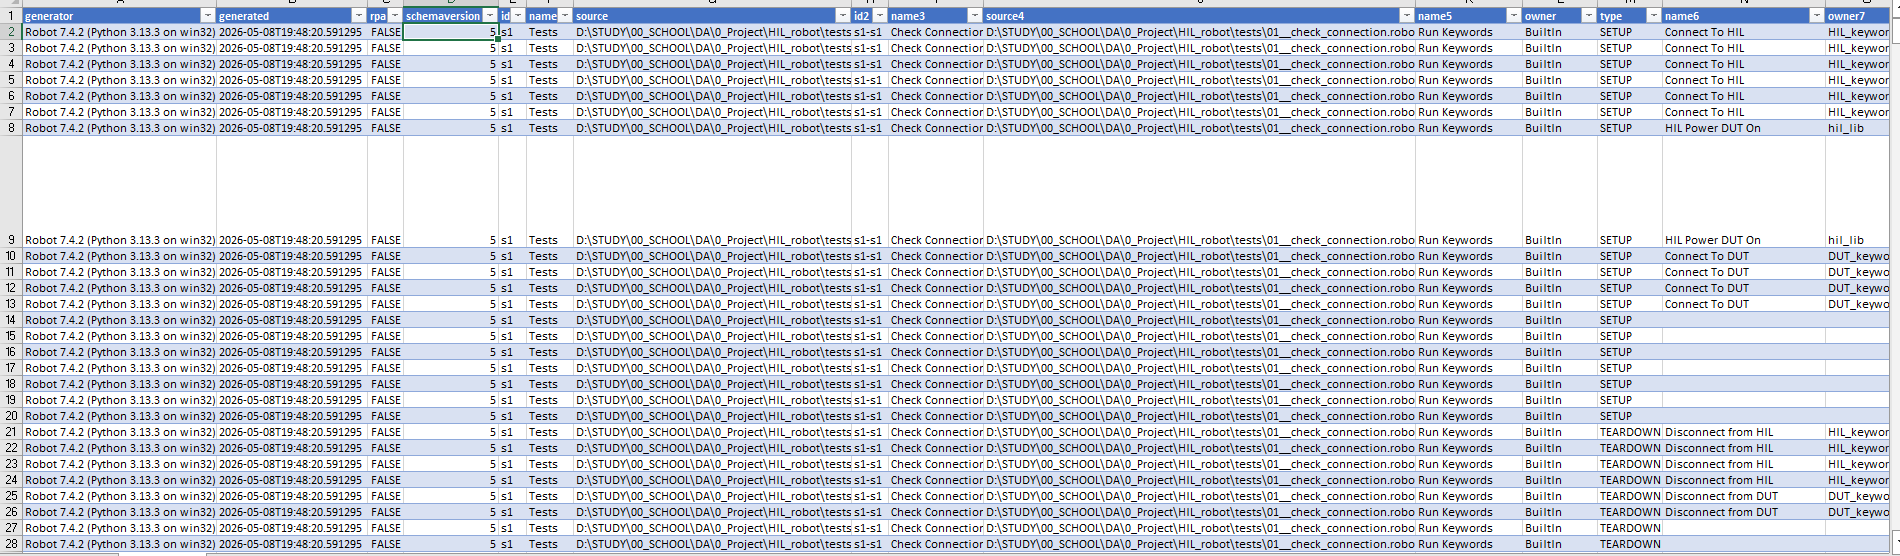
\includegraphics[width=0.85\textwidth]{image/robot_output.png}
    \caption{File output.xml chứa kết quả kiểm thử}
    \label{fig:robot_output_xml}
\end{figure}

File XML này cho phép hệ thống dễ dàng tích hợp với các công cụ xử lý kết quả kiểm thử hoặc các nền tảng tự động hóa khác trong tương lai như hệ thống CI/CD hoặc dashboard giám sát kiểm thử.

\subsubsection{File log giao tiếp HIL}

Ngoài các báo cáo của Robot Framework, hệ thống còn tự động ghi lại toàn bộ quá trình giao tiếp giữa máy tính và HIL thông qua file log serial với định dạng:

\begin{center}
\textbf{hil\_serial\_<ngày\_giờ>.log}
\end{center}

File log này lưu lại các lệnh điều khiển đã gửi đến HIL, dữ liệu phản hồi từ firmware cũng như trạng thái hoạt động của các ngoại vi mô phỏng trong suốt quá trình kiểm thử. Các file log này được lưu trong thư mục \textit{hil\_logs/} của hệ thống nhằm hỗ trợ người phát triển theo dõi và phân tích chi tiết quá trình giao tiếp với HIL.

Ví dụ, khi thực hiện kiểm thử CAN, file log sẽ ghi lại quá trình gửi dữ liệu CAN buffer, phản hồi nhận được từ DUT cũng như dữ liệu truyền nhận thực tế trên bus CAN. Tương tự, đối với các bài kiểm thử ADC, UART, GPIO hoặc I2C, file log cũng lưu lại toàn bộ nội dung giao tiếp tương ứng.

Hình \ref{fig:hil_serial_log} trình bày một phần nội dung của file log giao tiếp giữa Robot Framework và HIL.

\begin{figure}[H]
    \centering
    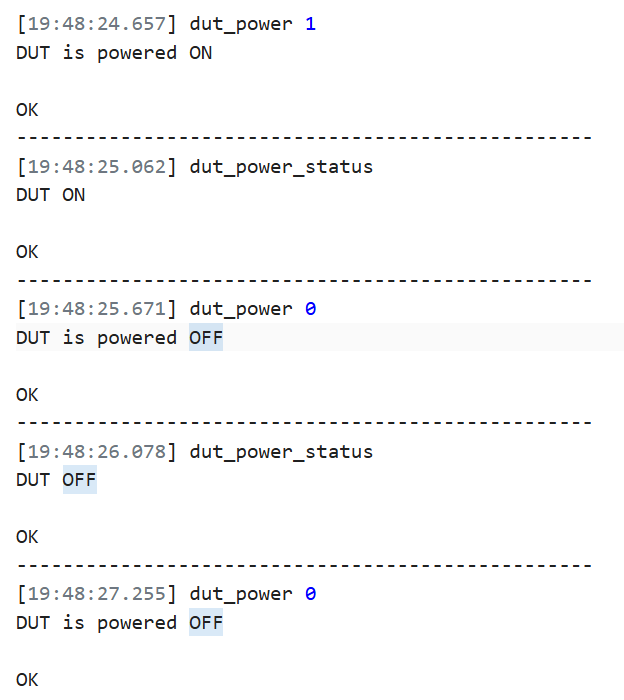
\includegraphics[width=0.85\textwidth]{image/hil_serial_log.png}
    \caption{File log giao tiếp serial giữa Robot Framework và HIL}
    \label{fig:hil_serial_log}
\end{figure}

Thông qua file log này, người phát triển có thể kiểm tra chính xác các lệnh đã được gửi xuống HIL cũng như dữ liệu phản hồi thực tế từ hệ thống phần cứng. Điều này đặc biệt hữu ích trong quá trình phân tích lỗi hoặc kiểm tra hoạt động của firmware DUT.

